% Standalone source; compile twice with pdflatex.
\documentclass{article}
\setlength{\paperwidth}{8.5in}
\setlength{\paperheight}{11in}
\setlength{\topmargin}{-0.75in}
\setlength{\headsep}{0in}
\setlength{\headheight}{0in}
\setlength{\evensidemargin}{-0.50in}
\setlength{\oddsidemargin}{-0.50in}
\setlength{\textwidth}{7.50in}
\setlength{\textheight}{10in}
\setlength{\parindent}{0in}
\setlength{\parskip}{0in}
\usepackage{amssymb,amsmath,amsthm,tikz,graphicx}
\usetikzlibrary{arrows.meta}
\usepackage{hyperref,fancyhdr,lastpage}
\hypersetup{colorlinks=true,urlcolor=blue,linkcolor=blue}
\urlstyle{same}
\pagestyle{fancy}
\fancyhf{}
\renewcommand{\headrulewidth}{0pt}
\rfoot{Page \thepage\hspace{1pt} of \pageref*{LastPage}}
\theoremstyle{plain}
\newtheorem{theorem}{Theorem}[section]
\newtheorem{example}{Example}[section]
\theoremstyle{definition}
\newtheorem{definition}{Definition}[section]
\theoremstyle{remark}
\newtheorem*{note}{Note}
\renewcommand{\vec}[1]{\mathbf{#1}}
\newcommand{\work}{\par\vfill}
\newcommand{\RHS}{\mathrm{RHS}}
\begin{document}
\begin{center}\huge The Simplex Method\end{center}
\section{Linear Programming and the Feasible Region}
\begin{definition}
A \textbf{linear programming problem} asks us to maximize or minimize a linear \textbf{objective function} subject to linear constraints. A \textbf{feasible solution} satisfies every constraint, including nonnegativity. The collection of feasible solutions is the \textbf{feasible region}; an \textbf{optimal solution} gives the best objective value on that region.
\end{definition}
\begin{theorem}
On a nonempty bounded feasible region defined by linear inequalities, a linear objective attains its maximum and minimum at vertices. More than one point may attain an optimum.
\end{theorem}
\begin{note}
These notes develop the simplex method for \emph{maximization} problems with constraints $A\vec{x}\le\vec{b}$, $\vec{x}\ge0$, and $\vec{b}\ge0$. The origin is then feasible. Problems requiring a different initial feasible basis need additional methods, which are outside this handout.
\end{note}
\begin{example}[Geometric interpretation]\label{ex:geometry}
Maximize $Z=4x+5y$ subject to
\[
\begin{cases}x+3y\le24,\\x-y\le4,\\x\le6,\end{cases}\qquad x,y\ge0.
\]
Sketch the feasible region, find its vertices, and use them to determine the maximum.
\end{example}
\medskip
\noindent\begin{minipage}[t]{0.48\textwidth}
\centering\textbf{The feasible region}\\[6pt]
\resizebox{\linewidth}{!}{\begin{tikzpicture}[x=0.66cm,y=0.66cm,>=Stealth,font=\small]
\draw[step=1,gray!18,very thin] (0,0) grid (9,9);
\fill[gray!15] (0,0)--(4,0)--(6,2)--(6,6)--(0,8)--cycle;
\draw[gray!65,dashed] (6,0)--(6,9);
\draw[gray!65] (0,8)--(9,5);
\draw[gray!65] (4,0)--(9,5);
\draw[very thick] (0,0)--(4,0)--(6,2)--(6,6)--(0,8)--cycle;
\draw[->,semithick] (0,0)--(9.8,0) node[right]{$x$};
\draw[->,semithick] (0,0)--(0,9.7) node[above]{$y$};
\foreach \k in {2,4,6,8}{
\draw (\k,0.08)--(\k,-0.08) node[below=3pt]{$\k$};
\draw (0.08,\k)--(-0.08,\k) node[left=3pt]{$\k$};}
\foreach \x/\y in {0/0,4/0,6/2,6/6,0/8}{\fill (\x,\y) circle (2.5pt);}
\node[below left=4pt] at (0,0) {$(0,0)$};
\node[above left=4pt] at (4,0) {$(4,0)$};
\node[right=6pt,fill=white,inner sep=2pt] at (6,2) {$(6,2)$};
\node[above right=5pt,fill=white,inner sep=2pt] at (6,6) {$(6,6)$};
\node[above right=4pt] at (0,8) {$(0,8)$};
\node[above,fill=white,inner sep=2pt] at (6,9) {$x=6$};
\node[right,fill=white,inner sep=2pt] at (8.1,5.65) {$x+3y=24$};
\node[right,fill=white,inner sep=2pt] at (8,3.7) {$x-y=4$};
\node[align=center] at (2.7,3.7) {Feasible\\region};
\end{tikzpicture}}
\end{minipage}\hfill
\begin{minipage}[t]{0.50\textwidth}
\centering\textbf{The objective function $Z=4x+5y$}\\[6pt]
\resizebox{\linewidth}{!}{\begin{tikzpicture}[x={(-0.40cm,-0.49cm)},y={(0.58cm,0cm)},z={(0cm,0.073cm)},>=Stealth,font=\small]
% Projection of the feasible region onto Z=0.
\fill[gray!10] (0,0,0)--(4,0,0)--(6,2,0)--(6,6,0)--(0,8,0)--cycle;
\draw[gray!65,thick] (0,0,0)--(4,0,0)--(6,2,0)--(6,6,0)--(0,8,0)--cycle;
% Vertical guides: each point rises to height 4x+5y.
\foreach \x/\y/\z in {4/0/16,6/2/34,6/6/54,0/8/40}{
\draw[gray!55,densely dashed] (\x,\y,0)--(\x,\y,\z);}
% The graph of the objective over the feasible polygon.
\draw[very thick] (0,0,0)--(4,0,16)--(6,2,34)--(6,6,54)--(0,8,40)--cycle;
\draw[->,semithick] (0,0,0)--(7.5,0,0) node[below left]{$x$};
\draw[->,semithick] (0,0,0)--(0,9.6,0) node[right]{$y$};
\draw[->,semithick] (0,0,0)--(0,0,63) node[above]{$Z$};
\foreach \k in {10,20,30,40,50,60}{
\draw (0,-0.10,\k)--(0,0.10,\k);
\node[left=4pt] at (0,0,\k) {$\k$};}
\foreach \x/\y in {4/0,6/2,6/6,0/8}{\fill[gray!65] (\x,\y,0) circle (2pt);}
\foreach \x/\y/\z in {0/0/0,4/0/16,6/2/34,6/6/54,0/8/40}{\fill (\x,\y,\z) circle (2.5pt);}
\node[above left=5pt,fill=white,inner sep=1pt] at (0,0,0) {$(0,0,0)$};
\node[below left=4pt] at (4,0,0) {$(4,0,0)$};
\node[below left=5pt] at (6,2,0) {$(6,2,0)$};
\node[below right=5pt] at (6,6,0) {$(6,6,0)$};
\node[below right=5pt] at (0,8,0) {$(0,8,0)$};
\node[below left=5pt,fill=white,inner sep=1pt] at (4,0,16) {$(4,0,16)$};
\node[above left=5pt,fill=white,inner sep=1pt] at (6,2,34) {$(6,2,34)$};
\node[above right=5pt,fill=white,inner sep=1pt] at (6,6,54) {$(6,6,54)$};
\node[above right=5pt] at (0,8,40) {$(0,8,40)$};
\end{tikzpicture}}
\end{minipage}
\smallskip
\begin{center}
\begin{tabular}{c|ccccc}
Vertex & $(0,0)$ & $(4,0)$ & $(6,2)$ & $(6,6)$ & $(0,8)$\\\hline
$Z=4x+5y$ & $0$ & $16$ & $34$ & $54$ & $40$
\end{tabular}
\end{center}
{\small In the right-hand graph, the gray polygon lies in $Z=0$; the black polygon consists of the points $(x,y,4x+5y)$. Dashed lines join corresponding vertices. The maximum is $Z=54$ at $(6,6)$.\par
\smallskip
\textit{This is an oblique projection: compare the labelled $Z$-coordinates, since vertical position on the page also depends on $x$.}\par}
\smallskip

\newpage
\section{Slack Variables and the Initial Tableau}
\begin{definition}
For a constraint $a_1x_1+\cdots+a_nx_n\le b$, introduce a \textbf{slack variable} $s\ge0$ and write
\[
a_1x_1+\cdots+a_nx_n+s=b.
\]
The slack is $s=b-(a_1x_1+\cdots+a_nx_n)$. It measures unused capacity when the constraint represents a resource. A constraint is \textbf{binding} when its slack is zero.
\end{definition}
Write $Z=c_1x_1+\cdots+c_nx_n$ as $-c_1x_1-\cdots-c_nx_n+Z=0$. The \textbf{simplex tableau} records the constraints and this objective equation, with right-hand sides in the last column. We retain an explicit $Z$ column.
\begin{definition}
For $m$ constraint rows, choose $m$ \textbf{basic variables} whose columns form the identity matrix in those rows and have zeros in the objective row. The other decision and slack variables are \textbf{nonbasic}. Set nonbasic variables to zero; the basic values can then be read from the right-hand side. If they are nonnegative, this is a \textbf{basic feasible solution}.
\end{definition}
\begin{note}
The objective column is also a unit column, but $Z$ records the objective value and is not counted among the $m$ basic decision/slack variables. Initially, the slacks form the basis.
\end{note}
\begin{example}\label{ex:setup}
For Example~\ref{ex:geometry}, add slack variables and build the initial tableau with columns $x,y,s_1,s_2,s_3,Z$. Read the initial basic feasible solution.
\end{example}

\work

\newpage
\section{Pivoting and the Stopping Rule}
For our objective-row convention, the current tableau represents an equation of the form
\[
Z+\sum_j r_j u_j=Z_0,
\]
where the $u_j$ are the nonbasic variables. Thus $Z=Z_0-\sum_jr_ju_j$.
\begin{theorem}[Optimality test]
If a tableau represents a basic feasible solution and all coefficients $r_j$ in its objective row are nonnegative, the current solution is optimal: every feasible choice has $u_j\ge0$, so $Z\le Z_0$.
\end{theorem}
\textbf{One pivot.}
\begin{enumerate}
\item Choose a negative variable coefficient in the objective row. In these examples, choose the \textbf{most negative} coefficient; its column is the entering-variable column.
\item In the constraint rows only, compute $\RHS/a$ for \textbf{strictly positive} entries $a$ in that column. Ignore zero and negative entries. A zero ratio is allowed.
\item The smallest ratio selects the pivot row and the leaving basic variable. The pivot is the entry at the intersection of the chosen row and column.
\item Divide the entire pivot row by the pivot, including its right-hand side.
\item Use that row to make all other entries in the pivot column zero, including the objective-row entry. Keep the other basic columns intact.
\item Repeat until the optimality test holds. Read the variables and verify the original constraints and objective.
\end{enumerate}
\begin{note}
A negative objective-row coefficient suggests a direction for improvement; a zero minimum ratio may give a pivot with no immediate gain. For these examples, ties may be resolved by the first eligible row. A systematic anti-cycling rule is needed for a general termination guarantee in degenerate problems.
\end{note}
\begin{example}\label{ex:firstsimplex}
Use the simplex method on the problem from Example~\ref{ex:geometry}. Show the ratio tests, every pivot operation, the optimal solution, and all slack values.
\end{example}

\work

\newpage
\textbf{Example 3.1 (continued).} Complete the simplex iterations and interpret the final tableau.

\work

\newpage
\begin{example}[Three decision variables]\label{ex:threevars}
Maximize
\[
Z=3x_1+5x_2+2x_3
\]
subject to
\[
\begin{cases}2x_1-x_2+3x_3\le6,\\x_1+2x_2+4x_3\le8,\end{cases}\qquad x_1,x_2,x_3\ge0.
\]
Use the simplex method and report the maximizing vector, objective value, and slack variables.\end{example}

\work

\newpage
\textbf{Example 3.2 (continued).} Complete the iterations and check the result.

\work

\newpage
\section{An Application: Allocating Aircraft}
\begin{example}\label{ex:airline}
A Montreal airline allocates aircraft to daily round trips to Toronto, Calgary, and Vancouver. Let $t,c,v$ be the numbers allocated to the three destinations. The daily profit is
\[
Z=400t+360c+450v.
\]
Each assigned aircraft requires the following staff:
\begin{center}\renewcommand{\arraystretch}{1.4}
\begin{tabular}{l|cc}
Destination & Pilots & Flight attendants\\\hline
Toronto & 2 & 4\\Calgary & 3 & 6\\Vancouver & 3 & 8
\end{tabular}\end{center}
There are 18 aircraft, 56 pilots, and 120 flight attendants available.
\begin{enumerate}
\item[(a)] Formulate the constraints and initial simplex tableau.
\item[(b)] Find an allocation that maximizes daily profit.
\item[(c)] Explain the slack variables in terms of unused resources.
\end{enumerate}
\end{example}
\begin{note}
Simplex treats the variables as real numbers. Aircraft allocations must ultimately be integers. If the optimal linear-programming solution is integral, it also solves this integer allocation problem; otherwise further work is required.
\end{note}

\work

\newpage
\textbf{Example 4.1 (continued).} Solve the allocation problem and interpret unused capacity.

\work

\newpage
\section{Additional Practice from the Supplied Notes}
\begin{example}\label{ex:practice3}
Maximize $Z=2x-y+z$ subject to
\[
\begin{cases}-x+5y-2z\le10,\\2x+y-z\le5,\\x-y+2z\le4,\end{cases}\qquad x,y,z\ge0.
\]
Use the simplex method, retaining exact fractions. Give the optimal vector, the maximum, and all slack values.
\end{example}

\work

\newpage
\textbf{Example 5.1 (continued).} Complete the pivots and verify all constraints.

\work

\newpage
\begin{example}[Four decision variables]\label{ex:practice4}
Maximize $Z=x+2y+3z+w$ subject to
\[
\begin{cases}2x+y+z\le18,\\3x+y+2z+3w\le36,\\x+z\le12,\end{cases}\qquad x,y,z,w\ge0.
\]
Use the simplex method and interpret the final tableau.
\end{example}

\work

\newpage
\textbf{Example 5.2 (continued).} Complete the iterations and check your answer.

\work

\newpage
\section*{Simplex Checklist}
\begin{enumerate}
\item \textbf{State the model.} Identify the decision variables, the objective, each inequality, and all nonnegativity conditions.
\item \textbf{Check the starting form.} For the method here, maximize with $\le$ constraints and nonnegative right-hand sides.
\item \textbf{Add slacks.} Use one distinct nonnegative slack for each constraint.
\item \textbf{Form the tableau.} Put the objective in the form $-c_1x_1-\cdots-c_nx_n+Z=0$. Keep a fixed column order.
\item \textbf{Choose an entering variable.} In these examples, use the most negative objective-row coefficient.
\item \textbf{Choose the leaving variable.} Compare right-hand side divided by a strictly positive pivot-column entry. Ignore zero and negative entries; retain zero ratios.
\item \textbf{Pivot.} Make the pivot $1$, then all other entries in its column $0$. Apply row operations to every entry, including the right-hand side and objective row.
\item \textbf{Stop and interpret.} Once all variable coefficients in the objective row are nonnegative, set nonbasic variables to zero and read the basic values and $Z$.
\item \textbf{Verify.} Substitute into every original constraint and the objective. Explain each slack in context.
\end{enumerate}
\begin{note}
If an entering column has a negative objective coefficient but no strictly positive entry in any constraint row, the objective is \textbf{unbounded above} from the current feasible tableau. There is no eligible leaving variable; do not invent a ratio using a zero or negative denominator.
\end{note}
\begin{note}
The ratio test preserves feasibility: increasing the entering variable by $\theta\ge0$ changes basic variable $i$ from $b_i$ to $b_i-a_i\theta$. If $a_i>0$, nonnegativity requires $\theta\le b_i/a_i$. The smallest eligible ratio is therefore the largest permissible step before some basic variable reaches zero.
\end{note}
\begin{note}
Do not round tableau entries prematurely. A unit-looking column alone is not enough to read a decision variable as basic: track the chosen basis and check that its objective-row coefficient is zero.
\end{note}
\vfill

\work

\newpage
\section{Dawson Final Examination Practice}
These prompts are reworded from the cited examinations, with their mathematical data retained. All decision variables are taken to be nonnegative.
\begin{example}[Fall 2024, Question 13]\label{ex:dawsonfall}
Use the simplex method to maximize
\[
Z=6x_1+2x_2+8x_3
\]
under the conditions
\[
\begin{cases}x_1+3x_2+x_3\le9,\\x_1+6x_2-x_3\le2,\\2x_2+x_3\le5,\end{cases}\qquad x_1,x_2,x_3\ge0.
\]
\end{example}
{\small\textit{Source:} Dawson College, 201-MA3-DW, \href{https://www.dawsoncollege.qc.ca/mathematics/wp-content/uploads/sites/113/Fall-2024-3.pdf}{Fall 2024 final examination}, Question 13, p. 15 (7 marks).}

\work

\newpage
\textbf{Example 6.1 (continued).} Finish the optimization and check the answer.

\work

\newpage
\begin{example}[Winter 2024, Question 12]\label{ex:dawsonwinter}
Use the simplex method to maximize $Z=2x-y+4z$ subject to
\[
\begin{cases}y+z\le30,\\2x-y+2z\le80,\\2x-y-z\le10,\end{cases}\qquad x,y,z\ge0.
\]
\end{example}
{\small\textit{Source:} Dawson College, 201-MA3-DW, \href{https://www.dawsoncollege.qc.ca/mathematics/wp-content/uploads/sites/113/Winter-2024-3.pdf}{Winter 2024 final examination}, June 3, 2024, Question 12, p. 12 (7 marks). Nonnegativity is made explicit here, consistently with the examination's intended simplex formulation.}

\work

\newpage
\textbf{Example 6.2 (continued).} Complete the simplex method and verify the maximum.

\work
\end{document}
